\epigraph{The epigraph for this chapter is left as an exercise to the reader}{}


\section{Structure of Assessments}

% How exams work - when they are - what are the weights of assessments and grades like? Subject to change per year so look at module informatio on blackboard 

% how to manage revision - asking for help, etc. 

% Speical cons policy for exams - add links 

% Mid-terms and finals 

Assessment in the first year is usually a mixture of coursework and written or online exams. The exact weighting varies between modules, so it’s always worth checking the information provided on Blackboard or the module page at the start of the semester. Lecturers will usually explain the assessment structure in the first few weeks of the module as well.

All first year modules also have a written in-person exam at the end of the semester. These typically take place during the university’s official exam periods which is in January for Semester 1 modules and in the summer for Semester 2 modules.

\section{Revision}
% how to revise well for something like maths? signpost to student hub learning skills and confidence and other helpful stuff available at uni. 

\subsection{Using Past Papers}
% how to use past papers effectivley? - don't just have the solutions as you do the papers, cuz there are dangers to that 
% tips for multiple choice - eliminate options 
% once you look at the solution, don't just gloss over it 
% also, don't rely on it as the only form of revision 

Past papers are one of the most useful revision tools you have, but also one of the easiest to misuse. 

It's very tempting to just load up a paper, try a question for a few minutes, get stuck, look at the solution, understand it and move on. The most important thing is to give yourself time to think before reaching for help. So if and when you don't know how to start a question, sit with it for a bit. Even if you don't solve it completely, that thinking time matters and it's what builds the ability to approach unfamiliar problems. 

If you look at a solution, try to reconstruct the proof yourself without looking. If you can't, that's a sign you didn't fully understand it yet, and that's fine. 

Try to not let past papers become the syllabus. It can be easy to fall into the habit of revision from the papers instead of using them as a tool to test your understanding. Exams don't always test whether you've seen a question before, but whether you understand the material well enough to deal with something slightly unfamiliar. So if your revision is entirely based on past papers, a small variation in a problem can make it feel like you've never seen it before.

\subsection{Dealing with Stress}
% Shakespeare in love - philip henslowe
% What to do if you're bored in an exam/deal with not wantiang to be there? 
% What to do if you're stressed the hell out in the exam

There is a particular kind of stress that arrives a few days before exams begin, and it’s not really about content. It’s about doubt.

You start asking questions that don’t have neat answers. Have I revised enough? What if I’ve focused on the wrong topics? What if the paper goes badly? What if I’ve misunderstood something fundamental? What if…? what if…? what if…? 

The mind becomes very creative under pressure. At some point it stops being about mathematics and starts being about catastrophe. Exam stress, dread, and self doubt are incredibly common, especially among people who care deeply about their subject. But even knowing that, it’s easy to feel alone when you’re in the middle of it.

I remember feeling this intensely before my first January exams in Semester 1. I was convinced I hadn’t done enough, that I was about to fail half my modules, and those thoughts seemed to be louder than any rational argument I could make.

I fondly remember speaking to my tutor about how stressed I was, and one of the first things he said to me was: 

\begin{quote}
    \textit{''It’s gonna to be alright. I’m not saying you’re gonna feel alright about it. I’m just saying it’s gonna to be alright."}
\end{quote}

I asked him how he knew, to which would response was, \textit{``How? I don’t know. It’s a mystery."}

Then he showed me a \textbf{\href{https://youtu.be/-hxTrm34oRI?si=08GXYMDkDqyzMvLp}{clip from Shakespeare in Love}}, where Philip Henslowe says exactly that line when everything seems to be falling apart.

Watching an 18 second YouTube video wasn’t exactly the kind of reassurance I expected going into that conversation, but there was something oddly comforting about that phrase. Something about it stayed with me, and it wasn’t because it removed the stress (it didn’t) but rather that it removed the demand to know, to predict, to control. It wasn’t saying I wouldn’t worry, but that uncertainty doesn’t mean catastrophe.

Later that evening, I printed out the script from Shakespeare in Love and put it on my wall. Since then, every time my mind started racing or I felt like I was catastrophising scenarios, I would look at it and smile, slightly against my will.

I don’t think the lesson here is that exams should feel easy, or that stress can be eliminated entirely. The lesson, at least for me, was simpler than that.

You revise as well as you can, sit the paper, and attempt the questions in front of you with whatever you can bring to mind that day.

Going in with that mindset feels very different from walking into the exam convinced you’re either going to ace everything, or on the flip side convinced you’re going to fail everything. Both extremes are unhelpful: one sets you up for pressure, the other for panic. 

Whereas if you accept that you don’t know exactly how it will go, and that you might surprise yourself in either direction, you can focus on thinking clearly instead of predicting the outcome.

And once the paper leaves your hands, some part of it really is a mystery.



\subsection{Comparison}
% This is not a rat race, cooperation over comparison or whatever else... talk abotu how comparison can cause anxiety, especially with Maths 

Comparison is one of the fastest ways to drain your confidence during revision. 

You will overhear conversations about how much or how many hours someone else has done, see people in the library morning to night, or someone say how they've completed every past paper twice. 

None of that gives you actual useful information. You don't know how well they understood the material, or what their starting point was, or even whether what they are telling you is the entire truth or only a fraction of it. 

The only revision that matters is yours. There will always be someone who appears more prepared, more calmer, or understands things instantly. Just because someone else appears better or smarter than you, doesn't make you any more or less good. Someone else understanding a concept quickly does not make you any less capable. 

The person who seems completely calm might also be unsure, and the student who answers questions confidently in lectures might have struggled with a different topic entirely. Nobody every has it `all worked out'. Comparison is always based on partial information, you rarely get to see the full picture. And during revision when anxiety and adrenaline are already elevated, comparison amplifies doubt without adding any insight. 

Mathematics is not a race in a straight line. Intellectual growth is personal, and often invisible. So let other people exist, let them be brilliant and revise in their way. You task is not to outperform everyone, but to engage the best you can with the material in front of you. 

\section{Results}
% in case things don't go according to plan - link to special cons. 
% Summer resits and criteria around that - add links to relevant things. 
% How first year grades don't count towards final degree- you just need to pass so don't stress too much blah blah blah - it's not an exuces for doing badly and not showing up to lectures tho 

% Section on addressing imposter syndrome thoughts like, “oh I don’t deserve these results because I didn’t work hard enough” and on the flip side, “I worked so hard only to get these low grades I'm terrible” 

During exams you’re busy thinking, writing, calculating, trying to make sense of questions under time pressure. But once the results come out, the thinking changes. You’re no longer solving problems but instead interpreting a number and trying to decide what it means about you.

The reaction to good results isn’t always excitement, sometimes it’s thoughts like  `Did I actually deserve that?' Or `I didn’t work hard enough to deserve that grade'. It’s that strange feeling of somehow getting away with something.

If you’ve ever had that thought, you’re not alone. Mathematics has a way of making people doubt themselves even when things go well. The subject constantly shows you how much more there is to learn, so it’s easy to feel like you’re always a step behind. But you’re allowed to accept the result you earned, you’re allowed to have done better than you expected.

The opposite reaction can happen too. Sometimes you work incredibly hard and the result feels disappointing and that can be much harder to process. When you’ve put hours into something, it’s easy to let one number turn into a judgement about your ability.

That voice can be very convincing in the moment. Remember that results are merely a snapshot of how things went in a particular exam, on a particular day, under particular conditions. It’s easy to believe that the world is like a neat function, that the effort your input always results in the outcome you want, but the world is uncertain and full of variables beyond our control. That doesn’t mean your effort was wasted, it just means your effort isn’t the only deciding factor, and it definitely doesn’t mean your worth is defined by one exam or one outcome. 

In first year especially, it’s worth keeping a bit of perspective. The marks from first year don’t count towards your final degree as long as you pass the modules. Now, that doesn’t mean the year doesn’t matter. It absolutely does, in fact, it’s where a lot of the real learning happens and it does count for any placements or internships you might want to apply. But it does mean the stakes aren’t quite as catastrophic as your brain might try to convince you.

If things genuinely don’t go according to plan, there are formal processes in place like summer resits, \textbf{\href{https://www.southampton.ac.uk/studentservices/academic-life/special-considerations.page}{special considerations}}, etc. It’s always worth checking in with your tutor following results if you find yourself in that situation. 


\begin{figure}[H]
    \centering
    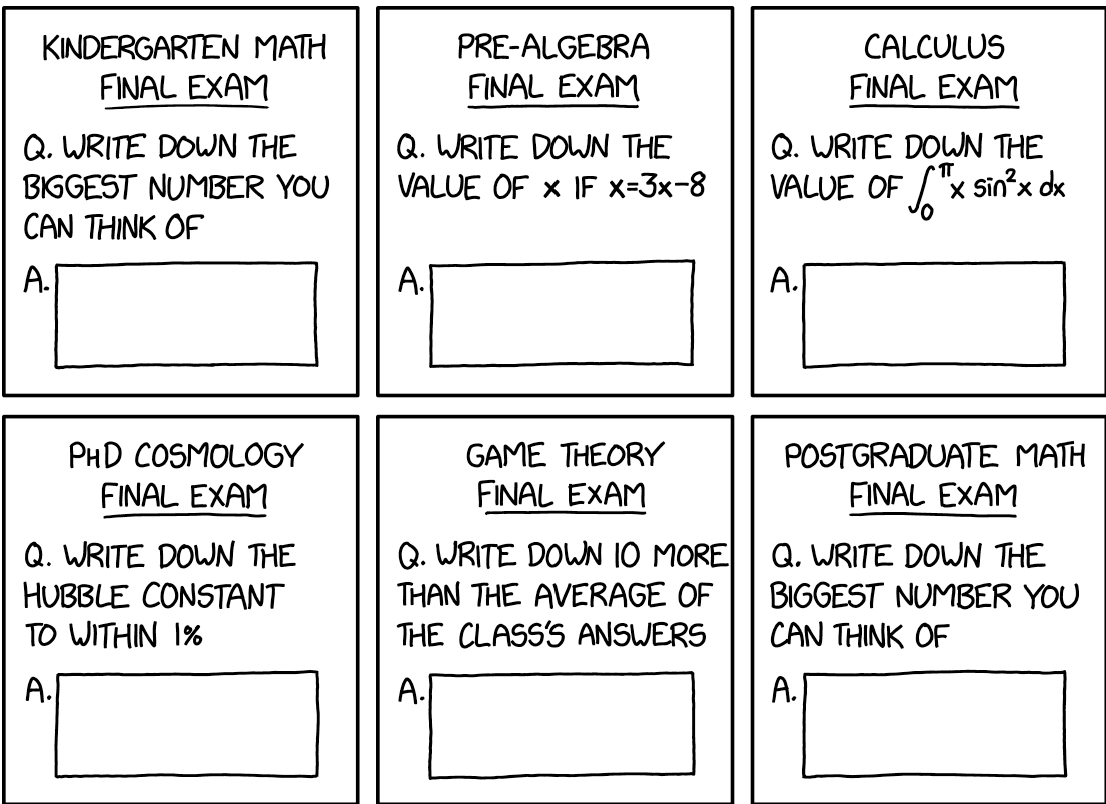
\includegraphics[width=0.5\linewidth]{xkcd/examNumbers.png}
    \caption{\textbf{\href{https://xkcd.com/2966/}{Exam Numbers}}}
\end{figure}


\begin{figure}[H]
    \centering
    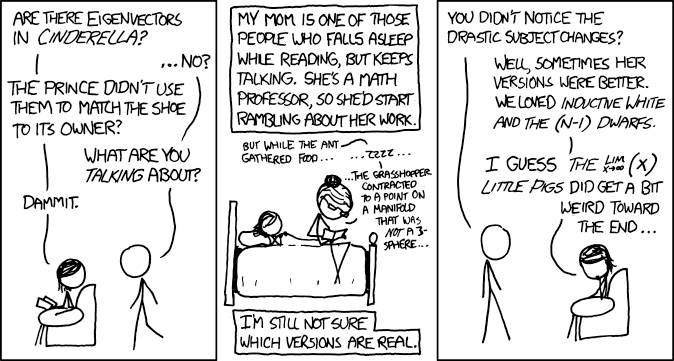
\includegraphics[width=0.6\linewidth]{xkcd/fairyTales.png}
    \caption{\textbf{\href{https://xkcd.com/872/}{Fairy Tales}}}
\end{figure}